\section{Architektur}
Wir beschreiben im Folgenden die Architektur von helios, die derzeit wie in Abbildung ~\ref{fig:hardarchitecture} konzipiert ist: helios fungiert als Vermittlungsschicht zwischen dem Spiel als Echtzeit-Datenmodell~\cite[525]{Gre19} und der technischen Infrastruktur.
Das Framework visualisiert den Spielzustand und überträgt Eingabedaten als Steuerkommandos an das Spiel weiter.

\begin{figure}[!h]
    \centering
    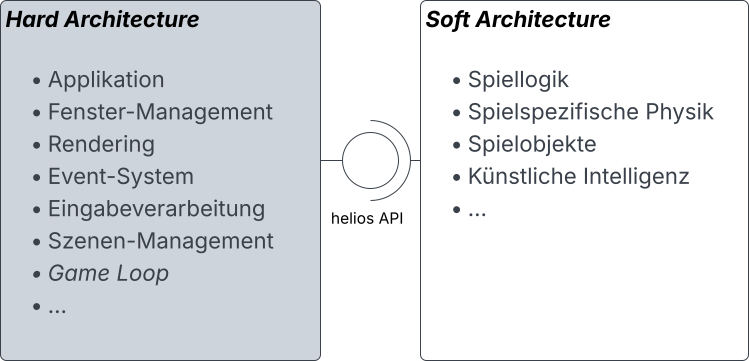
\includegraphics[width=1\columnwidth]{img/hardarchitecture.svg}
    \caption{Aufteilung der Architektur des helios Frameworks in \textit{Hard} und \textit{Soft Architecture} nach Rollins und Morris~\cite[612 ff.]{RM04}. Die Ball-/Socket-Notation deutet an, dass helios Schnittstellen zur Verfügung stellt, die ein (beliebiges) Spiel nutzen kann. (Quelle: eigene)}
    \label{fig:hardarchitecture}
\end{figure}

In Abbildung~\ref{fig:package_diagram} ist eine detailliertere Sicht auf die Module und ausgewählte Komponenten dargestellt.
Die Verzeichnisstruktur von helios spiegelt die Gliederung seiner Kernfunktionalitäten wider.
Im Sinne von \textit{Evans} ist dies entscheidend für eine hohe Kohäsion: Die Verzeichnisnamen kommunizieren die enthaltenen Funktionalitäten~\cite[180 f.]{Eva03}.
Innerhalb der Module findet eine weitere Unterteilung nach Schichten statt (etwa \texttt{controller}), was insgesamt als ``package-by-feature und -by-layer`` bezeichnet wird.


\begin{figure*}[t]
    \centering
    \makebox[\textwidth][c]{% Box ist textbreit, Inhalt darf überstehen
    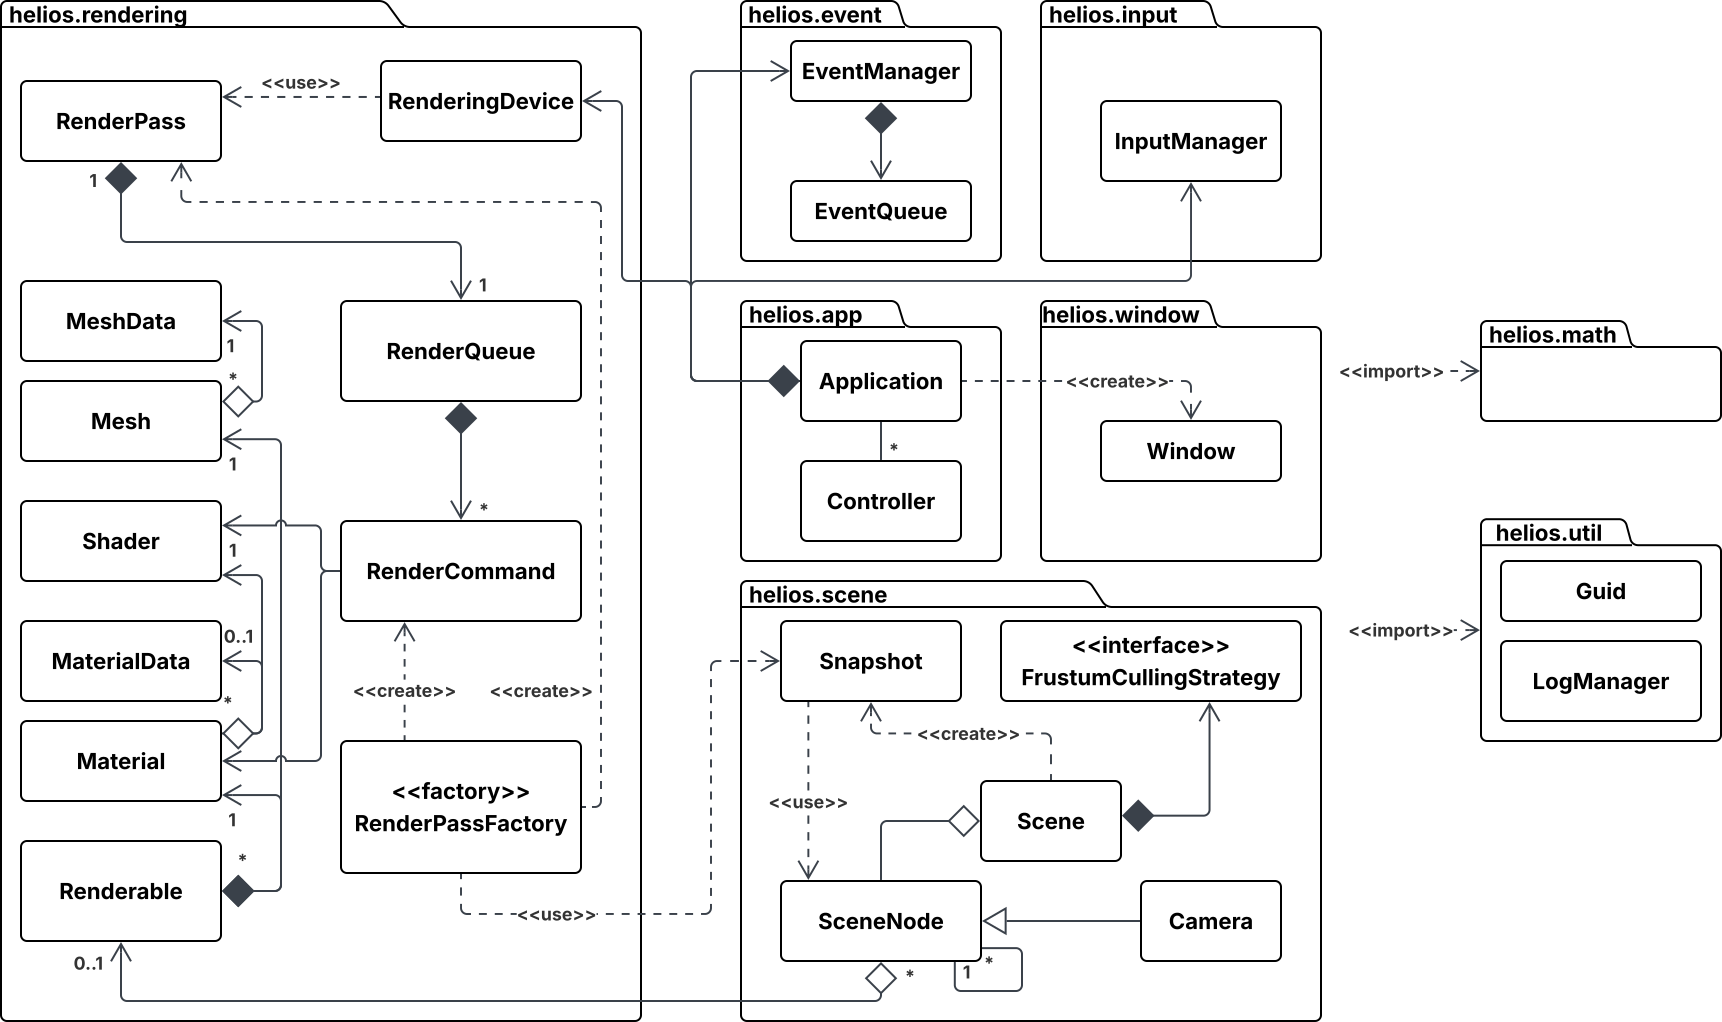
\includegraphics[width=1.4\textwidth]{img/package_diagram.svg}% \linewidth == Spaltenbreite
    }
    \caption{Aufbau des helios Framework und der Zusammenhang ausgewählter Komponenten. Die Strukturierung der Module orientiert sich an einem ``by Feature, by Layer``-Konzept. (Quelle: eigene)}

    \label{fig:package_diagram}

\end{figure*}


\subsection*{\texttt{app}: Applikationsschicht}
Die zentrale Steuereinheit der Anwendung bzw. des Spiels bildet die Klasse \texttt{Application}, die über Event-System, Eingabeverarbeitung und Fenstermanagement verfügt sowie das Rendering-Backend - repräsentiert durch \texttt{RenderDevice} - initialisiert.\par
helios unterstützt an dieser Stelle außerdem dynamisches Hinzufügen von Applikations-Controllern~\cite[379]{Fow03} zur Definition isolierter, ereignisbasierter Steuerungslogik, beispielsweise dem Verhalten bei einem Window-Resize\footnote{
Die Applikations-Controller wurden ursprünglich eingeführt, um ``Framebuffer-Resize``-Ereignisse gegenüber dem Rendering-Backend zu abstrahieren.
}.

\subsection*{\texttt{input}: Eingabeverarbeitung}
Der \texttt{InputManager} orchestriert die Eingabeverarbeitung.
Er wird ausschließlich von der Anwendung verwaltet und an das aktive Fenster gebunden.\par
Ein spezialisierter \texttt{InputAdapter} abstrahiert von den durch die TPLs bereitgestellten Eingabeereignissen und übersetzt sie für den \texttt{InputManager}.
Zu Beginn der Game Loop werden aktive Eingabeereignisse gepollt (\texttt{InputManager::poll()}). Eine Abfrage der Ereignisse erfolgt über Methoden wie \texttt{InputManager::isKeyPressed()}.

\subsection*{\texttt{event}: Ereignisverarbeitung}
Ereignisse können über den \texttt{EventManager} in eine \texttt{EventQueue} geschrieben werden (``post``).
Interessierte Beobachter (\textit{Observer}) können sich über Callbacks mittels \texttt{subscribe} bei dem \texttt{EventManager} registrieren~\cite[293 ff.]{GHJV94}.
Die Methode \texttt{EventManager::dispatchAll()} informiert die Observer über vorhandene Ereignisse.

\subsection*{\texttt{window}: Fensterklasse}
Die \texttt{Window}-Klasse stellt Schnittstellen zur Steuerung des Anwendungsfensters, zur Abfrage von Fensterereignissen und zur Anweisung des \textit{Buffer-Swappings} bereit.


\subsection*{\texttt{math}: Mathematische Typen und Operationen}
Dieses Modul stellt im Namespace \texttt{helios::math} trigonometrische Funktionen und Repräsentanten für in der Linearen Algebra verankerte Datentypen wie Vektoren und Matrizen bereit.
Es unterstützt außerdem Operationen für lineare und affine Transformationen und realisiert damit den in der  3D-Computergrafik gebräuchlichen Koordinatenraumwechsel

\[
    \text{Model}\rightarrow\text{World}\rightarrow\text{View}\rightarrow\text{Projection}\rightarrow\text{Clip}
\]

\noindent

Die Schnittstellen orientieren sich bei den Methodensignaturen an populären Bibliotheken wie dem bereits erwähnten \texttt{glm}.

\subsection*{\texttt{scene}: Szenengraph}
Der Szenengraph \texttt{helios::scene::Scene} folgt etablierten Implementierungen aus der Literatur\footnote{siehe unter anderem~\cite[]{She07} sowie~\cite[]{Gre19}}.
\texttt{Scene} besitzt einen impliziten Wurzelknoten, der eine beliebige Anzahl von Kindknoten enthalten kann.
Jeder \texttt{SceneNode} verfügt über ein \texttt{Transform}-Objekt, das die Modelltransformation im lokalen Koordinatensystem beschreibt.\par
\texttt{SceneNodes} können ``darstellbar`` sein, das heißt, sie sind mit einem \texttt{Renderable} konfiguriert.
Sie können aber auch einfach nur eine Kamera (\texttt{helios::scene::Camera}) repräsentieren\footnote{oder positionierbare \texttt{LightNodes}, also Lichtquellen}.\par
Szenenknoten mit \texttt{Renderable} werden beim \textit{Culling} berücksichtigt.
Das Culling-Verfahren wird in der rein virtuellen Klasse \textit{FrustumCullingStrategy} abstrakt definiert. Spezialisierungen werden der \texttt{Scene} bei der Instanziierung übergeben.\par
In der Application Stage~\cite[687]{Gre19} erstellt helios aus einer Szene und einer Kamera einen \texttt{Snapshot}, für den die konfigurierte Culling-Strategie alle im sichtbaren Bereich der Kamera befindlichen \texttt{SceneNode}s sammelt.
Ein einzelner Snapshot bildet die Grundlage für einen \texttt{RenderPass}, der die nötigen Anweisungen (\texttt{RenderCommand}s) für den eigentlichen Rendering-Prozess enthält.
Listing~\ref{lst:gameloop} zeigt den Ablauf einer einfachen Game Loop.

\vspace{4mm}
\begin{lstlisting}[style=c++style, caption={Implementierung einer einfachen Game Loop in helios. Von der Szene wird ein \texttt{Snapshot} erstellt, der als Grundlage für den \texttt{RenderPass} dient.}, label=lst:gameloop]
while (!win->shouldClose()) {
  app->eventManager().dispatchAll();

  inputManager.poll(0.0f);

  if (inputManager.isKeyPressed(Key::ESC)) {
      win->setShouldClose(true);
  }

  snapshot   = scene->createSnapshot(*camera);
  renderPass = factory.buildRenderPass(
    snapshot
  );

  app->renderingDevice().render(renderPass);

  win->swapBuffers();
}
\end{lstlisting}
\vspace{4mm}


\subsection*{\texttt{rendering}: Render Pipeline}
Das Rendering-System von helios ist in verschiedene Module aufgeteilt, darunter \texttt{shader} für Shader/GLSL-spezifischen Code sowie \texttt{model} für Abstraktionen von Material- und Mesh-Daten.\par
\texttt{Renderable}s sind Repräsentanten ``darstellbarer`` Objekte.
Sie kapseln für den Rendering-Prozess notwendige Informationen und sind als Aggregation modelliert.
Sie bestehen aus individuell konfigurierbaren \texttt{Material}- und \texttt{Mesh}-Instanzen, die wiederum \texttt{MaterialData}- und \texttt{MeshData}-Objekte zur einfachen und ressourcenschonenden Wiederverwendung mit anderen Instanzen teilen~\cite[126]{AHHP+18}.\par

Die für einen \texttt{RenderPass} benötigten Informationen werden als \texttt{RenderCommand}-Objekte in einer \texttt{RenderQueue} gesammelt, die vom eigentlichen \texttt{RenderDevice} verarbeitet werden: \texttt{RenderCommand}s besitzen Zeiger auf die darzustellende Geometrie (\texttt{Mesh}), die zu nutzenden \texttt{Shader} sowie Daten-Objekte, in denen Informationen zu \texttt{Uniform}-Variablen (bspw. Transformationsmatrizen) gespeichert sind.\par
Das \texttt{RenderDevice} verarbeitet einen \texttt{RenderPass} über Template-Methoden \texttt{preRender, doRender} und \texttt{postRender}.


\subsection*{\texttt{util}: Utility-Klassen}
Im Modul \texttt{helios::util} liegt nicht-domänenspezifischer Code, wie der \texttt{LogManager} für einfache Logging-Funktionalitäten sowie eine \texttt{Guid}-Implementierung zur Konfiguration von Objekten mit einem globalen eindeutigen Identifikator (\textit{global unique identifier}).